%% ============================================================================
%%  UAGS: RA-L first submission (double-anonymous), RAS conference class.
%%  Assembled 2026-09-29 from the section drafts (front, related, method,
%%  experiments, preamble). Source of every claim: the 2026-09-29 fact sheet
%%  (docs/reports/2026-09-29-paper-revision-1/logs/fact_sheet.md); the code
%%  under usplat/ is the ground truth for every formula.
%%  Revised 2026-09-29 after the math, claims and form reviews (fix pass).
%%
%%  >>> READ ME BEFORE SUBMITTING <<<
%%  * Every number cell comes from a saved evaluation (see the %% comment above each
%%    table and docs/reports/2026-10-17-paper-completion). \ph / \todo are unused now.
%%  * Localization and active view selection (EFE) are not part of this paper.
%%    Their old text is parked in papers/parked_sections.tex, as is the old
%%    timing table and the old fourth contribution (one backward pass).
%%  * Build: tectonic main.tex (runs BibTeX itself). References: ref.bib, which also
%%    holds the IEEEtran.bst control entry (et al. rule).
%% ============================================================================
%% Fonts under tectonic (tectonic runs XeTeX, not pdfLaTeX).
%% IEEEtran selects Times with \rmdefault{ptm}. XeTeX's default text encoding
%% is TU, and there is no TU/ptm font. Without the next line the text silently
%% falls back to Latin Modern and \bfseries prints in regular weight.
%% T1 selects the URW Times Type 1 fonts (NimbusRomNo9L) that pdfLaTeX uses
%% for the reference PDF. It must come BEFORE \documentclass: the class
%% sets its display and paragraph skips in ex units while it loads, so it must
%% see Times then, as it does under pdfLaTeX (loaded later, these skips come
%% out about 4% too small).
%% Keep the .tex and .bib sources ASCII. Write accents as LaTeX commands
%% (e.g. {\'e}) and quotes as ``...''. T1 under XeTeX does not map Unicode
%% input: a typed curly quote prints as a wrong glyph.
\RequirePackage[T1]{fontenc}

%% RA-L is a JOURNAL, so the submission uses the IEEE journal template.
%% (This file briefly used ieeeconf, the ICRA/IROS conference class; that was
%% wrong for RA-L. \overrideIEEEmargins and \IEEEoverridecommandlockouts were
%% ieeeconf/conference-mode commands and are gone with it.)
\documentclass[journal]{IEEEtran}

%% ---------------------------------------------------------------------------
%% Packages
%% ---------------------------------------------------------------------------
\usepackage{amsmath,amssymb,amsfonts}
\interdisplaylinepenalty=2500 % IEEEtran advice after amsmath: lets align break pages
\usepackage{graphicx}
\usepackage{booktabs}
\usepackage{array}
\usepackage{textcomp}         % \textdegree and similar text symbols
\usepackage{algorithm}        % float wrapper for pseudo-code
\usepackage{algorithmic}      % \begin{algorithmic} ... \STATE ...
\usepackage[table]{xcolor}  % [table]: \cellcolor in the per-class table header
\usepackage{cite}             % sorted, compressed numeric citations [1]-[3]
%% amsthm clashes with ieeeconf: the class already defines \proof and
%% \endproof, so \usepackage{amsthm} stops with "Command \proof already
%% defined". If amsthm is ever needed, load it like this:
%\let\proof\relax
%\let\endproof\relax
%\usepackage{amsthm}
%% ieeeconf has its own \newtheorem style, so plain \newtheorem works without amsthm.
\usepackage{xr-hyper}          % references to the paper (main.aux)
\usepackage[colorlinks=true,allcolors=blue]{hyperref}  % load hyperref last
\externaldocument[M-]{main}
\hypersetup{pdfauthor={Anonymous Authors}}             % keep PDF metadata anonymous

%% IEEE reference style: more than six authors -> first author "et al.". IEEEtran.bst
%% reads the control entry IEEEexample:BSTcontrol (top of ref.bib) through \bstctlcite,
%% which IEEEtran.cls provides (called right after \begin{document}).
%% \bstctlcite comes from IEEEtran.cls, so it is not defined here any more.

%% ---------------------------------------------------------------------------
%% Draft macros (same as papers/main.tex)
%% ---------------------------------------------------------------------------
\newcommand{\todo}[1]{\textcolor{red}{\textbf{[TODO: #1]}}}
\newcommand{\ph}{\textcolor{red}{XX.X}}      % numeric placeholder
\newcommand{\phn}{\textcolor{red}{X}}        % integer placeholder
\newcommand{\R}{\mathbf{R}}
\newcommand{\xv}{\mathbf{x}}
\newcommand{\zv}{\mathbf{z}}
\newcommand{\muv}{\boldsymbol{\mu}}
\newcommand{\etav}{\boldsymbol{\eta}}
\newcommand{\Sph}{\mathbb{S}}
\newcommand{\reimpl}{\textsuperscript{$\dagger$}}   % re-implemented baseline row
\newcommand{\phs}{\ph{\scriptsize$\,\pm\,$\ph}}     % mean +- std placeholder
\newcommand{\secref}[1]{Sec.~\mbox{\ref{#1}}}       % keeps "III-F" on one line

%% ---------------------------------------------------------------------------
%% Title and anonymous byline (double-anonymous: no names, affiliations,
%% e-mails, funding, \thanks notes or acknowledgments)
%% ---------------------------------------------------------------------------
%% Title. The plan (2026-09-28-paper-completion-plan/1-plan.md, Sec. 6) ties the title to
%% the G2 grid; this is cell A. Swap once G2/G3 are measured:
%%   B (epistemic pass, calibration fail): Detecting and Forgetting Stale Open-Vocabulary
%%     Semantics in Gaussian Splatting with View-Level Evidence
%%   C (epistemic fail, calibration pass): Calibrated Open-Vocabulary Gaussian Splatting
%%     that Forgets Stale Semantics
%%   D (both fail): Detecting and Forgetting Stale Open-Vocabulary Semantics in Gaussian
%%     Splatting
\title{Supplementary Material:\\ Uncertainty-Aware Open-Vocabulary Gaussian Splatting for Changing Scenes}

%% Double-anonymous review: no names, affiliations, funding or links.
\author{Anonymous Authors}

%% Notes (from the template check):
%%  * IEEEtran provides IEEEkeywords and \IEEEPARstart. RA-L collects the
%%    keywords in the PaperCept form as well, so the block is optional for
%%    the first submission.
%%  * Last page: to balance the columns, put \addtolength{\textheight}{-Xcm}
%%    in the text of the last page (tune X by hand), as the official root.tex does.

\begin{document}
\bstctlcite{IEEEexample:BSTcontrol}
\maketitle
\renewcommand{\thesection}{S\arabic{section}}
\renewcommand{\thetable}{S\arabic{table}}
\renewcommand{\thefigure}{S\arabic{figure}}

This supplement accompanies the paper. Numbers of sections, tables and figures without the prefix S refer to the paper. Every number comes from a saved evaluation of the paper's protocol. The test scenes had been evaluated before the analyses of Sections~\ref{supp:stats}, \ref{supp:stale} and~\ref{supp:cost}, so their tests are descriptive; Section~\ref{supp:attempts} lists the later attempts to improve the results, each registered before it ran.

\section{Calibration and paired tests}
\label{supp:stats}
All test scenes were seen before these tests, so they are descriptive. For each baseline and metric of Table~\ref{M-tab:replica} we count the test scenes in which ours is better, take the median paired difference, and apply an exact two-sided sign test over the 14 scenes of both datasets, with Holm's correction over the 20 comparisons (Table~\ref{tab:paired}). Ours and averaging do not differ in any metric; ours is better than LEGaussians in every metric and has a lower NLL than Feature 3DGS and lower ECE, NLL and Brier than the 2D features in 13 of 14 scenes. Averaging and P0 have the same lead over the trained rows, so it comes from training-free lifting, not from the adaptive temperature. ECE also depends on how it is averaged (Table~\ref{tab:calib}, Fig.~\ref{fig:calibration}): over all test pixels pooled, P2 has the highest ECE of the open-vocabulary rows on Replica (7.1), while it has the lowest mean over scenes (8.7); its Brier score is the lowest under both.

\begin{table*}[t]
\centering
\caption{Ours against each baseline, paired over the test scenes (Replica $N=6$, ScanNet $N=8$). x/N: scenes in which ours is better (median paired difference in brackets; positive: ours better; points except NLL in nats). mIoU compares ours P0, the other columns ours P2. Sign test over the 14 scenes, Holm over the 20 tests (\textbf{bold}: below 0.05); Wilcoxon as a secondary column.}
\label{tab:paired}
\footnotesize
\setlength{\tabcolsep}{4pt}
\begin{tabular}{@{}llcccccc@{}}
\toprule
Baseline & Metric & Replica & ScanNet & Both & Median & Sign $p$ & Holm $p$ \,/\, Wilcoxon $p$\\
\midrule
%% generated by scripts/quant_stats.py (commands in docs/reports/2026-10-20-figures-video/logs/quant_summary.md)
Averaging & mIoU & 3/6 (-0.01) & 5/8 (0.00) & 8/14 & 0.00 & 0.79 & 1 \,/\, 0.86\\
Averaging & ECE & 3/6 (+0.32) & 3/8 (-0.18) & 6/14 & -0.18 & 0.79 & 1 \,/\, 0.71\\
Averaging & NLL & 5/6 (+0.009) & 4/8 (-0.002) & 9/14 & +0.006 & 0.42 & 1 \,/\, 0.36\\
Averaging & Brier & 6/6 (+0.38) & 4/8 (+0.02) & 10/14 & +0.24 & 0.18 & 1 \,/\, 0.17\\
Averaging & AURC & 6/6 (+1.24) & 0/8 (-0.49) & 6/14 & -0.09 & 0.79 & 1 \,/\, 0.86\\
\midrule
Feature 3DGS & mIoU & 2/6 (-0.17) & 7/8 (+1.85) & 9/14 & +0.49 & 0.42 & 1 \,/\, 0.078\\
Feature 3DGS & ECE & 4/6 (+0.42) & 7/8 (+1.24) & 11/14 & +0.81 & 0.057 & 0.46 \,/\, 0.0085\\
Feature 3DGS & NLL & 6/6 (+0.051) & 7/8 (+0.033) & 13/14 & +0.038 & 0.0018 & \textbf{0.033} \,/\, 0.0031\\
Feature 3DGS & Brier & 6/6 (+0.80) & 6/8 (+0.76) & 12/14 & +0.80 & 0.013 & 0.14 \,/\, 0.0052\\
Feature 3DGS & AURC & 6/6 (+1.80) & 6/8 (+0.16) & 12/14 & +0.69 & 0.013 & 0.14 \,/\, 0.0052\\
\midrule
LEGaussians & mIoU & 6/6 (+3.16) & 8/8 (+5.01) & 14/14 & +3.52 & 0.00012 & \textbf{0.0024} \,/\, 0.00012\\
LEGaussians & ECE & 6/6 (+1.14) & 8/8 (+1.58) & 14/14 & +1.26 & 0.00012 & \textbf{0.0024} \,/\, 0.00012\\
LEGaussians & NLL & 6/6 (+0.136) & 7/8 (+0.081) & 13/14 & +0.108 & 0.0018 & \textbf{0.033} \,/\, 0.00024\\
LEGaussians & Brier & 6/6 (+3.33) & 7/8 (+2.14) & 13/14 & +3.24 & 0.0018 & \textbf{0.033} \,/\, 0.00024\\
LEGaussians & AURC & 6/6 (+3.37) & 7/8 (+0.38) & 13/14 & +1.62 & 0.0018 & \textbf{0.033} \,/\, 0.0012\\
\midrule
2D features & mIoU & 4/6 (+1.05) & 7/8 (+5.43) & 11/14 & +3.45 & 0.057 & 0.46 \,/\, 0.0085\\
2D features & ECE & 5/6 (+3.50) & 8/8 (+2.67) & 13/14 & +3.21 & 0.0018 & \textbf{0.033} \,/\, 0.00061\\
2D features & NLL & 6/6 (+0.105) & 7/8 (+0.094) & 13/14 & +0.100 & 0.0018 & \textbf{0.033} \,/\, 0.00085\\
2D features & Brier & 6/6 (+3.77) & 7/8 (+3.55) & 13/14 & +3.56 & 0.0018 & \textbf{0.033} \,/\, 0.00037\\
2D features & AURC & 6/6 (+3.49) & 6/8 (+1.24) & 12/14 & +2.01 & 0.013 & 0.14 \,/\, 0.00061\\
\bottomrule
\end{tabular}
\end{table*}

\begin{table}[t]
\centering
\caption{Calibration under two aggregations: mean over the test scenes (as Table~\ref{M-tab:replica}) and pooled over all test pixels. ECE in \%, NLL in nats.}
\label{tab:calib}
\footnotesize
\setlength{\tabcolsep}{2.5pt}
\begin{tabular}{@{}lcccccccc@{}}
\toprule
& \multicolumn{4}{c}{Replica} & \multicolumn{4}{c}{ScanNet}\\
\cmidrule(lr){2-5}\cmidrule(l){6-9}
& \multicolumn{2}{c}{ECE} & \multicolumn{2}{c}{NLL} & \multicolumn{2}{c}{ECE} & \multicolumn{2}{c}{NLL}\\
Row & mean & pool & mean & pool & mean & pool & mean & pool\\
\midrule
%% generated by scripts/quant_stats.py (commands in docs/reports/2026-10-20-figures-video/logs/quant_summary.md)
Ours P2 & 8.70 & 7.12 & 0.996 & 0.982 & 6.06 & 2.62 & 0.509 & 0.506\\
Ours P0 & 9.86 & 5.62 & 0.996 & 0.981 & 6.36 & 3.16 & 0.510 & 0.502\\
Ours P1 & 10.21 & 8.69 & 1.039 & 1.022 & 6.97 & 3.59 & 0.522 & 0.508\\
Averaging & 9.62 & 5.70 & 1.004 & 0.989 & 6.17 & 3.13 & 0.512 & 0.499\\
Feature 3DGS & 10.01 & 6.29 & 1.044 & 1.028 & 7.38 & 4.72 & 0.571 & 0.553\\
LEGaussians & 10.59 & 6.20 & 1.136 & 1.121 & 8.10 & 4.63 & 0.628 & 0.605\\
2D features & 11.78 & 7.05 & 1.116 & 1.097 & 8.78 & 5.11 & 0.638 & 0.621\\
CSS (closed set) & 5.05 & 3.13 & 1.014 & 0.999 & 7.03 & 2.63 & 0.604 & 0.556\\
\bottomrule
\end{tabular}
\end{table}

\begin{figure*}[t]
  \centering
  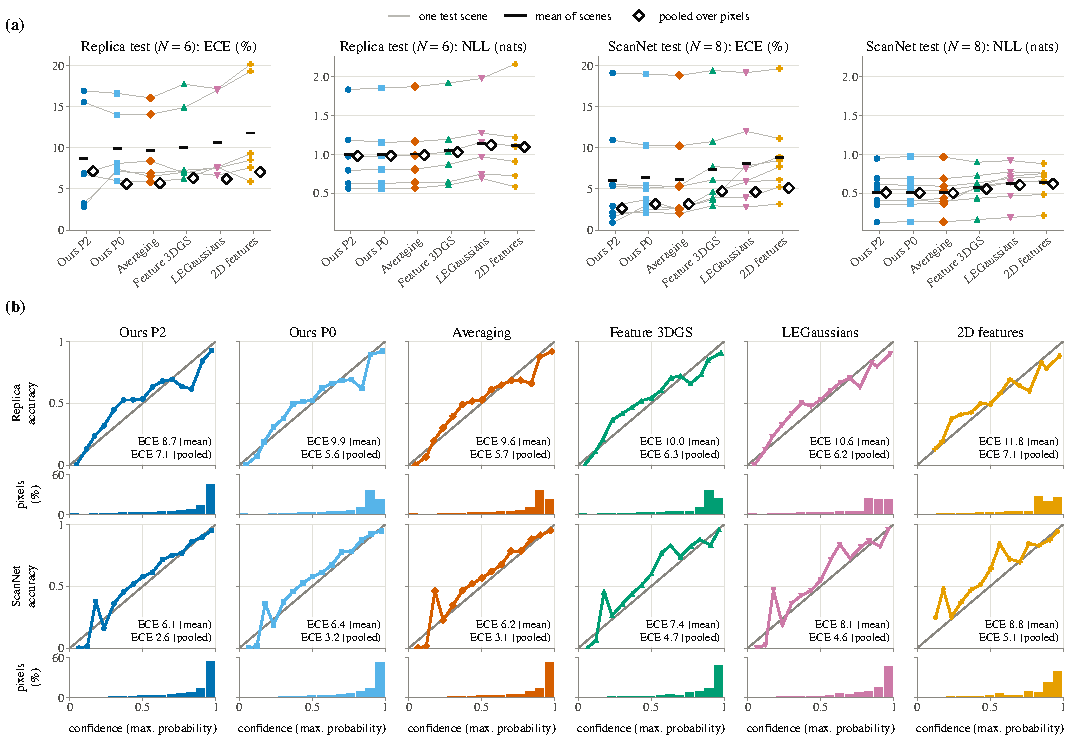
\includegraphics[width=\textwidth]{figs/calibration.pdf}
  \caption{Calibration on the test scenes. (a) ECE and NLL per scene (grey lines join the rows of one scene), their mean over scenes (bar) and the value pooled over all pixels (diamond). (b) Reliability diagrams pooled over the test pixels of each dataset (15 equal-width bins) with the share of pixels per bin.}
  \label{fig:calibration}
\end{figure*}


\section{Stale content}
\label{supp:stale}
\subsection{Fused baselines}
Table~\ref{tab:fused} repeats the fused rows of Table~\ref{M-tab:change} and tests our fused row against each by an exact sign test over the ten test scenes, with Holm's correction over the eight tests. The feature residual and NormLift's drop, fused with depth the same way as ours, rank the stale Gaussians better than our fused row.

%% NOR qualitative figures and fused baselines (2026-10-21): scripts/nor_qual.sh; every dump reproduces its
%% Table III record (docs/reports/2026-10-20-figures-video/logs/nor_summary.md); fused rows pre-registered in
%% configs/nor_fused_prereg.json (dae4b10) before any fused score; marks by make_tables.mark_columns.
\begin{table*}[t]
\centering
\caption{Every change row fused with the depth residual by the rank average of our fused row (pre-registered, run after Table~\ref{M-tab:change}), object-removal test scenes, mean $\pm$ std ($N=10$), \%. Bottom: our fused row against each, scenes in which ours is higher, median difference (points), sign test and Holm over the 8 tests.}
\label{tab:fused}
\footnotesize
\setlength{\tabcolsep}{5pt}
\begin{tabular}{@{}llcccc@{}}
\toprule
& & \multicolumn{2}{c}{Gaussian level} & \multicolumn{2}{c}{Pixel level}\\
\cmidrule(lr){3-4}\cmidrule(l){5-6}
Method & In & AP & AUROC & AP & AUROC\\
\midrule
Ours fused with depth residual & F+D & 75.0{\scriptsize$\,\pm\,$12.9} & 92.3{\scriptsize$\,\pm\,$2.9} & 61.8{\scriptsize$\,\pm\,$13.8} & \underline{78.2}{\scriptsize$\,\pm\,$11.3}\\
NCC photometric residual + depth & I+D & 61.2{\scriptsize$\,\pm\,$17.7} & 85.3{\scriptsize$\,\pm\,$9.4} & 56.8{\scriptsize$\,\pm\,$12.0} & 74.2{\scriptsize$\,\pm\,$12.3}\\
Feature residual, $k=2$, + depth & F+D & \textbf{81.1}{\scriptsize$\,\pm\,$9.4} & \underline{92.8}{\scriptsize$\,\pm\,$3.2} & \underline{64.3}{\scriptsize$\,\pm\,$13.4} & \underline{78.2}{\scriptsize$\,\pm\,$12.1}\\
NormLift reliability drop + depth & F+D & \underline{79.9}{\scriptsize$\,\pm\,$15.1} & \textbf{93.9}{\scriptsize$\,\pm\,$2.4} & \textbf{66.9}{\scriptsize$\,\pm\,$12.2} & \textbf{79.6}{\scriptsize$\,\pm\,$12.1}\\
Dispersion $1-\hat\rho$ + depth & F+D & 34.2{\scriptsize$\,\pm\,$8.7} & 82.5{\scriptsize$\,\pm\,$5.3} & 35.8{\scriptsize$\,\pm\,$22.2} & 61.7{\scriptsize$\,\pm\,$16.2}\\
\midrule
Ours + depth vs & Level & Higher & Median & Sign $p$ & Holm $p$\\
\midrule
NCC photometric residual & Gaussian AP & 9/10 & +10.9 & 0.021 & 0.107\\
NCC photometric residual & Pixel AP & 8/10 & +7.4 & 0.109 & 0.328\\
Feature residual, $k=2$ & Gaussian AP & 0/10 & -1.2 & 0.002 & 0.016\\
Feature residual, $k=2$ & Pixel AP & 3/10 & -0.6 & 0.344 & 0.344\\
NormLift reliability drop & Gaussian AP & 1/10 & -1.7 & 0.021 & 0.107\\
NormLift reliability drop & Pixel AP & 2/10 & -4.8 & 0.109 & 0.328\\
Dispersion $1-\hat\rho$ & Gaussian AP & 10/10 & +41.2 & 0.002 & 0.016\\
Dispersion $1-\hat\rho$ & Pixel AP & 10/10 & +25.5 & 0.002 & 0.016\\
\bottomrule
\end{tabular}
\end{table*}

\subsection{Measured false-alarm rate}
\label{supp:rstatic}
The threshold targets a per-view false-alarm rate of $10^{-3}$ on static content (\secref{M-sec:change}). Table~\ref{tab:rstatic} gives the measured rate $r_{\mathrm{static}}$, the share of the tests on static observed Gaussians during the update that fire, for every row at its own label-free threshold. Ours has a median of $4.0\times10^{-3}$ over the ten test scenes, within a factor of two of nominal in one scene; it is closer to nominal than the feature residual, NCC, the dispersion and NormLift's drop in 10, 9, 9 and 8 of the ten scenes, and less close than the depth residual (3 of 10).

\begin{table*}[t]
\centering
\caption{Measured per-view false-alarm rate on static Gaussians, $r_{\mathrm{static}}$ ($\times10^{-3}$; nominal 1), on the object-removal scenes. Median (min--max) over the ten test scenes, pooled over them, validation median, median $\lvert\log_{10}(r_{\mathrm{static}}/10^{-3})\rvert$, test scenes within a factor of two of nominal, and test scenes in which ours is closer to nominal than the row.}
\label{tab:rstatic}
\footnotesize
\begin{tabular}{@{}lcccccc@{}}
\toprule
Row & Test median (range) & Test pooled & Val. median & $\lvert\log_{10}\rvert$ & Within $2\times$ & Ours closer\\
\midrule
%% generated by scripts/quant_stats.py (commands in docs/reports/2026-10-20-figures-video/logs/quant_summary.md)
NCC photometric residual & 22.2 (1.1--204.9) & 32.1 & 32.9 & 1.35 & 1/10 & 9/10\\
Depth residual & 1.1 (0.3--9.1) & 2.6 & 1.6 & 0.40 & 3/10 & 3/10\\
Feature residual, $k=2$ & 52.8 (4.3--277.8) & 71.0 & 68.0 & 1.72 & 0/10 & 10/10\\
NormLift reliability drop & 4.1 (0.1--191.0) & 50.7 & 6.6 & 0.90 & 0/10 & 8/10\\
Dispersion $1-\hat\rho$ (ours) & 8.3 (3.0--68.4) & 28.8 & 2.3 & 0.91 & 0/10 & 9/10\\
Ours: test, reset, re-admission & 4.0 (0.5--23.4) & 3.6 & 4.8 & 0.60 & 1/10 & --\\
\bottomrule
\end{tabular}
\end{table*}


\subsection{Qualitative results and stale answers}
Fig.~\ref{fig:qual-change} renders every change score on three test scenes chosen by a fixed rule, and Fig.~\ref{fig:qual-query} shows how the semantics of a text query change over the update. The stale-answer rate of \secref{M-sec:exp-change} is the share of the removed object's covered pixels, over all update keyframes, whose top class over the 101 Replica classes is the scene's query (the most frequent top class of the stale Gaussians after mapping, computed by rule).

\begin{figure*}[t]
  \centering
  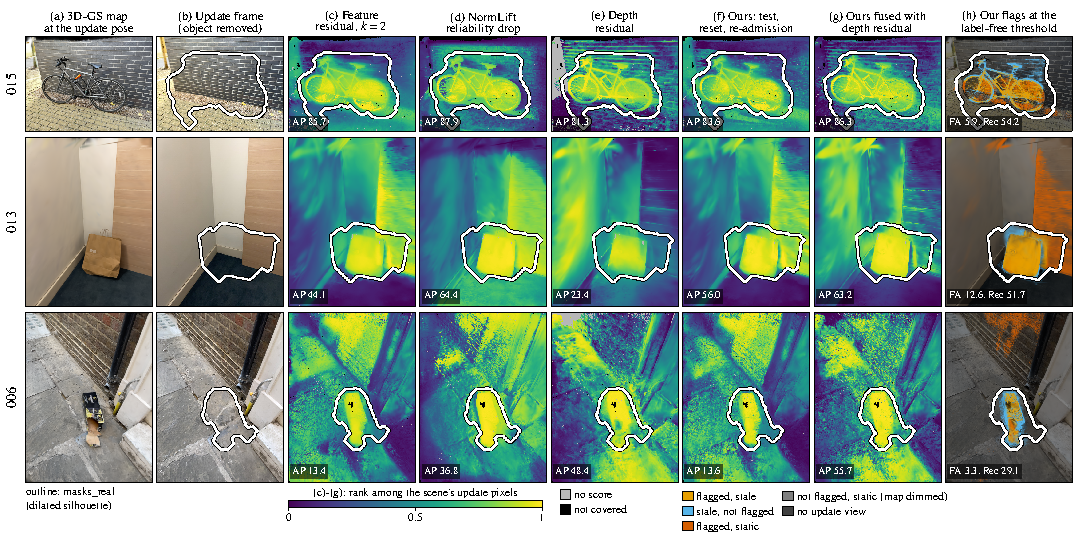
\includegraphics[width=\textwidth]{figs/qual_change.pdf}
  \caption{Stale content after a real removal (NeRF-Object-Removal test scenes 015 at frame 675, 013 at frame 556, 006 at frame 178). The scenes are fixed by rule: the highest, the lower-median and the lowest pixel-level AP of ours in Table~\ref{M-tab:change}; the frame is the update keyframe with the largest object region inside the image. The map geometry is fixed: (a) renders the map, so the removed object's Gaussians are still there; (b) is the camera image after the removal. (c)-(g) render each row's per-Gaussian score, coloured by its rank among the covered pixels of all update keyframes of the scene (the population of the pixel-level AP; grey: no score, black: not covered); the numbers are the rows' pixel-level AP (\%) in Table~\ref{M-tab:change}. (h) shows our flags at the label-free threshold against the stale Gaussians (orange: flagged and stale, light blue: stale and not flagged, vermillion: flagged and static), with FA/Rec.\ (\%) of ours counted over all update views (015 5.9/54.2, 013 12.6/51.7, 006 3.3/29.1). The outline is masks\_real, a dilated silhouette of the object. NormLift's drop has a higher pixel-level AP than our test in all three scenes, as in Table~\ref{M-tab:change} (9 of 10 test scenes).}
  \label{fig:qual-change}
\end{figure*}

\begin{figure*}[t]
  \centering
  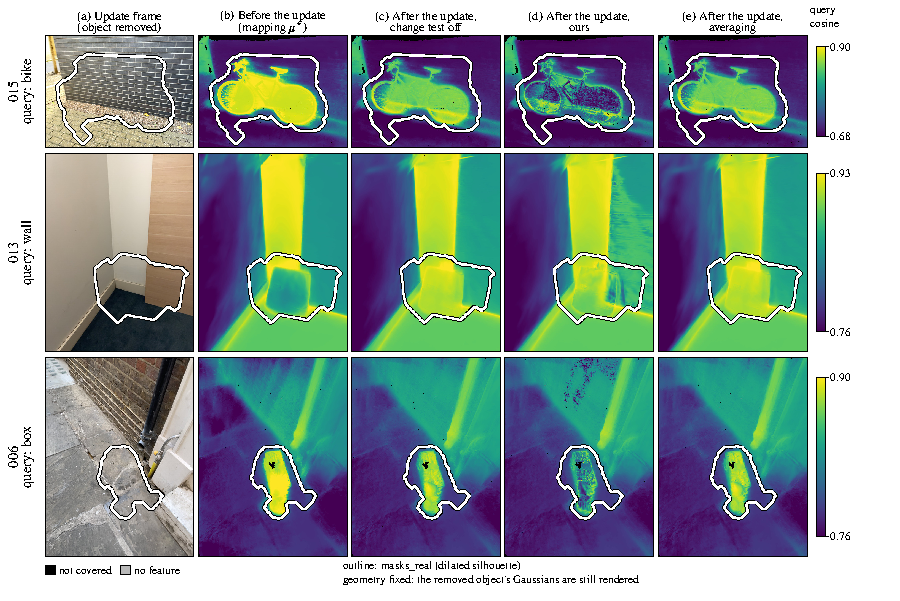
\includegraphics[width=\textwidth]{figs/qual_query.pdf}
  \caption{Query relevance before and after the update, same scenes, frames and rotations as Fig.~\ref{fig:qual-change}. The query of each scene is fixed by rule and never re-prompted: the most frequent top class (101 Replica classes, LSeg 5-template ensemble) of the mapping-pass $\boldsymbol\mu^\star_n$ of the stale Gaussians (015: 'bike', 013: 'wall', 006: 'box'). Each panel shows the cosine between the rendered feature and the query text, one colour scale per row (5th to 99th percentile of (b)). The map geometry is fixed: the removed object's Gaussians are still rendered after the update and only their semantics change. (c) is the same field after the same update views with the change test off; (d) is ours, where only the Gaussians our test flags are reset (Rec.\ 54.2/51.7/29.1\% in these scenes), so the missed ones keep the old class; (e) is averaging. The outline is masks\_real, a dilated silhouette.}
  \label{fig:qual-query}
\end{figure*}

\section{Static scenes: per class and per method}
\label{supp:static}
Fig.~\ref{fig:qual} shows both uncertainties on a Replica test frame. Table~\ref{tab:perclass} gives the per-class IoU of the rows of Table~\ref{M-tab:replica}. On Replica, ours leads on ceiling and chair, and the other rows lead elsewhere by 0.1 to 2.1 points. On ScanNet, ours leads on cabinet, chair and bed and ties on window, while averaging leads on floor, wall and door by 0.2 to 0.4 points. Fig.~\ref{fig:qual-compare} compares every method on one test frame of each dataset, and Fig.~\ref{fig:supp-grid} on one frame of every test scene; scenes and frames follow rules fixed before rendering.

%% Uncertainty figure (user request 2026-10-19): scripts/render_qual.py, room_0 (test),
%% evaluation frame 29 = the frame with the most e_red pixels (--list-frames, rule fixed
%% before rendering); 30-frame field mapped as in scripts/replica_views.sh (--max-keyframes 30);
%% meta /home/thanhnc/gauss_ws/src/uags/results/qual/qual_room_0_f29.json
\begin{figure*}[t]
  \centering
  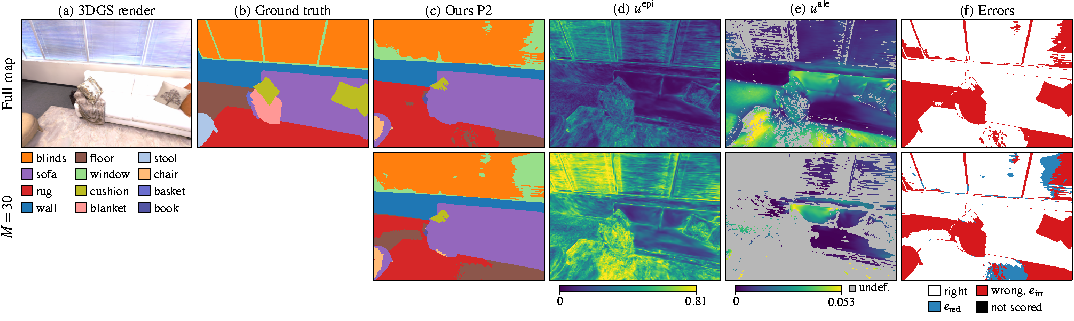
\includegraphics[width=\textwidth]{figs/qual.pdf}
  \caption{Uncertainty on a Replica test frame (room\_0, the evaluation frame with the most reducible-error pixels). Top: the full map; bottom: a field from $M=30$ of the 180 mapping frames on the same geometry. (c) labels of P2, (d) $u^{\mathrm{epi}}$, (e) $u^{\mathrm{ale}}$ (grey: undefined, fewer than $\tau_{\min}$ views), (f) right and wrong pixels; at $M=30$ the wrong pixels split into reducible ($e_{\mathrm{red}}$, blue) and irreducible ($e_{\mathrm{irr}}$, red) errors. With 30 frames, $u^{\mathrm{epi}}$ rises, also where the reducible errors are, while $u^{\mathrm{ale}}$ is still undefined on most pixels; with the full map, $u^{\mathrm{ale}}$ is highest at the rug, where the labels stay wrong.}
  \label{fig:qual}
\end{figure*}

%% Per-class IoU (user requests 2026-10-19/20, layout of CSS's Table I): generated by
%% scripts/make_tables.py perclasspair eval_test_224fe1e.json --val eval_val_224fe1e.json --pair
%% scannet_tab1/eval_test.json scannet_tab1/eval_val.json (classes in >= 5 scenes of each dataset);
%% log docs/reports/2026-10-17-paper-completion/logs/perclasspair_rows.tex
\begin{table*}[t]
\centering
\caption{Per-class IoU (\%) on the Replica ($N=6$) and ScanNet ($N=8$) test scenes for the classes in at least five scenes (mean over the scenes with the class; on Replica, vent and wall-plug score 0 for every row and are left out). mIoU: over all classes (Table~\ref{M-tab:replica}). Marks per dataset as in Table~\ref{M-tab:replica}; an IoU of 0 is not marked; CSS is not ranked.}
\label{tab:perclass}
\footnotesize
\setlength{\tabcolsep}{3pt}
\begin{tabular}{@{}l*{9}{c}|c@{\hspace{8pt}}*{7}{c}|c@{}}
\toprule
& \multicolumn{10}{c}{Replica} & \multicolumn{8}{c}{ScanNet}\\
\cmidrule(lr){2-11}\cmidrule(l){12-19}
Method & \cellcolor[HTML]{1F78B4}\rotatebox{90}{\textcolor{white}{ceiling}} & \cellcolor[HTML]{B15928}\rotatebox{90}{\textcolor{white}{door}} & \cellcolor[HTML]{6A3D9A}\rotatebox{90}{\textcolor{white}{floor}} & \cellcolor[HTML]{8C564B}\rotatebox{90}{\textcolor{white}{lamp}} & \cellcolor[HTML]{2F4F4F}\rotatebox{90}{\textcolor{white}{wall}} & \cellcolor[HTML]{E31A1C}\rotatebox{90}{\textcolor{white}{chair}} & \cellcolor[HTML]{33A02C}\rotatebox{90}{\textcolor{white}{panel}} & \cellcolor[HTML]{D95F02}\rotatebox{90}{\textcolor{white}{table}} & \cellcolor[HTML]{7570B3}\rotatebox{90}{\textcolor{white}{window}} & \rotatebox{90}{\textbf{mIoU}} & \cellcolor[HTML]{6A3D9A}\rotatebox{90}{\textcolor{white}{floor}} & \cellcolor[HTML]{2F4F4F}\rotatebox{90}{\textcolor{white}{wall}} & \cellcolor[HTML]{1B9E77}\rotatebox{90}{\textcolor{white}{cabinet}} & \cellcolor[HTML]{B15928}\rotatebox{90}{\textcolor{white}{door}} & \cellcolor[HTML]{E31A1C}\rotatebox{90}{\textcolor{white}{chair}} & \cellcolor[HTML]{B8860B}\rotatebox{90}{\textcolor{white}{bed}} & \cellcolor[HTML]{7570B3}\rotatebox{90}{\textcolor{white}{window}} & \rotatebox{90}{\textbf{mIoU}}\\
\midrule
2D features, per frame & 78.9 & 47.0 & 46.9 & \underline{25.2} & 75.9 & 63.2 & 0.0 & 51.3 & 12.3 & 26.3 & 88.6 & 79.1 & 66.1 & 56.3 & 58.5 & 80.4 & 54.0 & 62.5\\
Averaging~\cite{joseph2025gradbp}\reimpl & 80.5 & \textbf{60.0} & \underline{49.6} & 22.4 & \underline{78.0} & \underline{70.0} & 0.0 & \textbf{53.8} & \underline{15.6} & \underline{27.9} & \textbf{90.3} & \textbf{81.6} & \underline{71.6} & \textbf{67.3} & \underline{68.9} & \underline{89.7} & \textbf{57.0} & \underline{67.7}\\
Feature 3DGS~\cite{zhou2024feature}\reimpl & \underline{80.8} & 59.2 & \textbf{49.7} & 25.0 & \textbf{78.1} & 65.6 & 0.0 & 52.4 & \textbf{17.1} & \underline{27.9} & 89.7 & 81.0 & 69.6 & 62.6 & 63.9 & 83.6 & \underline{55.7} & 65.0\\
LEGaussians~\cite{shi2024legaussians}\reimpl & 79.0 & 52.5 & 45.8 & \textbf{25.9} & 75.7 & 58.9 & \textbf{0.1} & 48.4 & \underline{15.6} & 24.0 & 88.3 & 78.7 & 66.6 & 56.7 & 59.9 & 81.5 & 53.3 & 62.3\\
Ours (P0 and P2 share labels) & \textbf{80.9} & \underline{59.7} & 49.3 & 23.8 & \underline{78.0} & \textbf{70.7} & 0.0 & \underline{53.1} & \underline{15.6} & \textbf{28.0} & \underline{90.1} & \underline{81.3} & \textbf{72.0} & \underline{66.9} & \textbf{70.4} & \textbf{90.1} & \textbf{57.0} & \textbf{68.0}\\
\midrule
CSS~\cite{wilson2025css}\reimpl, closed set & 80.5 & 54.9 & 50.3 & 27.0 & 78.3 & 68.6 & 0.0 & 54.1 & 16.2 & 28.5 & 90.5 & 82.1 & 72.4 & 68.3 & 66.5 & 88.8 & 57.1 & 67.3\\
\bottomrule
\end{tabular}
\end{table*}

%% Static comparison (2026-10-21): scripts/qual_compare.sh figures; rules and test looks in
%% docs/reports/2026-10-20-figures-video/logs/static_summary.md; numbers read from the Table I JSONs.
\begin{figure*}[t]
  \centering
  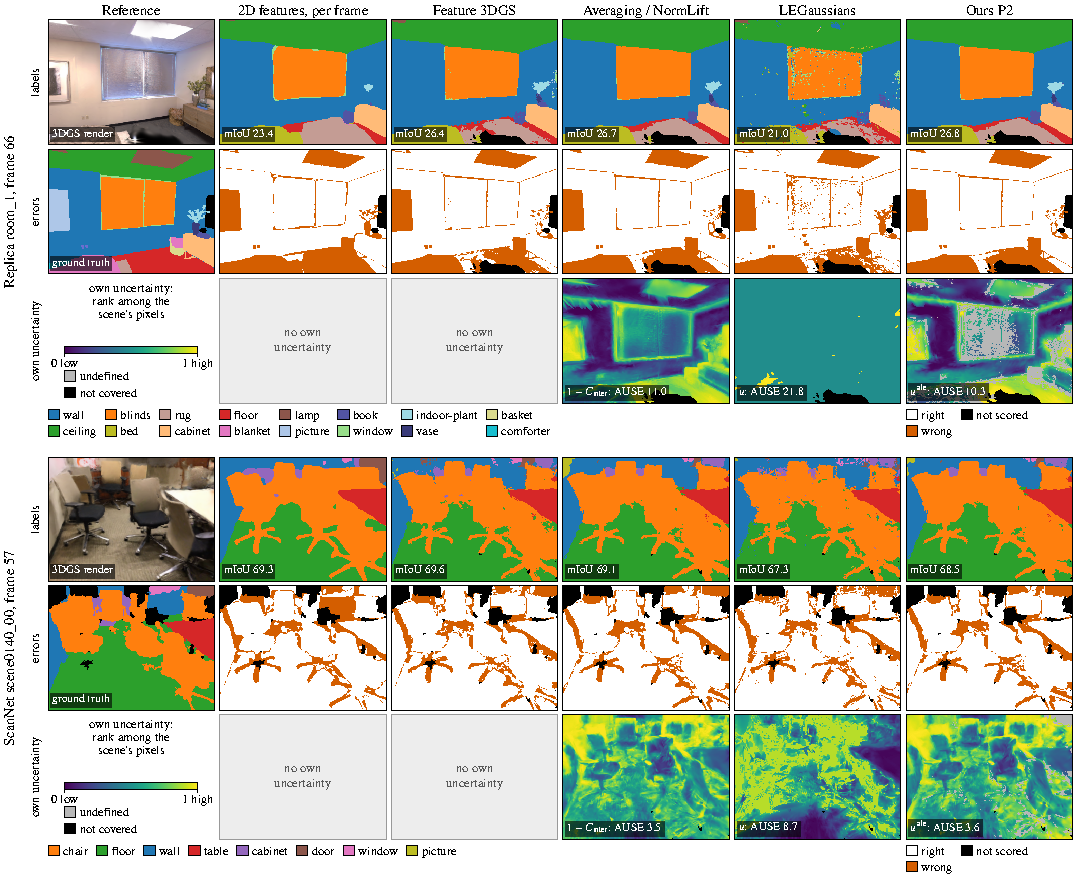
\includegraphics[width=\textwidth]{figs/qual_compare.pdf}
  \caption{Segmentation and own uncertainty of every method on Replica room\_1 (frame 66) and ScanNet scene0140\_00 (frame 57). Each scene is the test scene with the lower-median per-scene mIoU of ours P2 in Table~\ref{M-tab:replica}, and each frame is the evaluation frame with the most ground-truth classes that cover at least 0.5\% of its labeled pixels; both rules read only the published table and the labels and were fixed before rendering. Row 1: the 3DGS render and the labels (black: no decision); row 2: the ground truth and the errors (vermillion: wrong; black: not scored); row 3: each method's own uncertainty, NormLift's $1-C_{\mathrm{inter}}$, the learned $u$ of LEGaussians and our $u^{\mathrm{ale}}$, as its rank among the covered labeled pixels with a defined value in all evaluation frames of the scene (grey: undefined; black: not covered). The 2D features and Feature 3DGS have no own uncertainty (-- in Table~\ref{M-tab:replica}); we show no P2 confidence. Numbers are per-scene values over all evaluation frames, read from Table~\ref{M-tab:replica}: mIoU (row 1) and the AUSE of the own uncertainty (row 3), in \%. LEGaussians $\lambda_u$ = 4 (Replica), 1 (ScanNet), chosen on validation. On room\_1, ours has the highest mIoU (26.8). On room\_1, $u^{\mathrm{ale}}$ has the lowest AUSE of the own uncertainties (10.3 vs 11.0, 21.8). On scene0140\_00, ours (68.5 mIoU) is below Feature 3DGS (69.6), the 2D features (69.3) and averaging (69.1). On scene0140\_00, NormLift's $1-C_{\mathrm{inter}}$ ranks the errors slightly better than $u^{\mathrm{ale}}$ (AUSE 3.5 vs 3.6).}
  \label{fig:qual-compare}
\end{figure*}

\begin{figure*}[p]
  \centering
  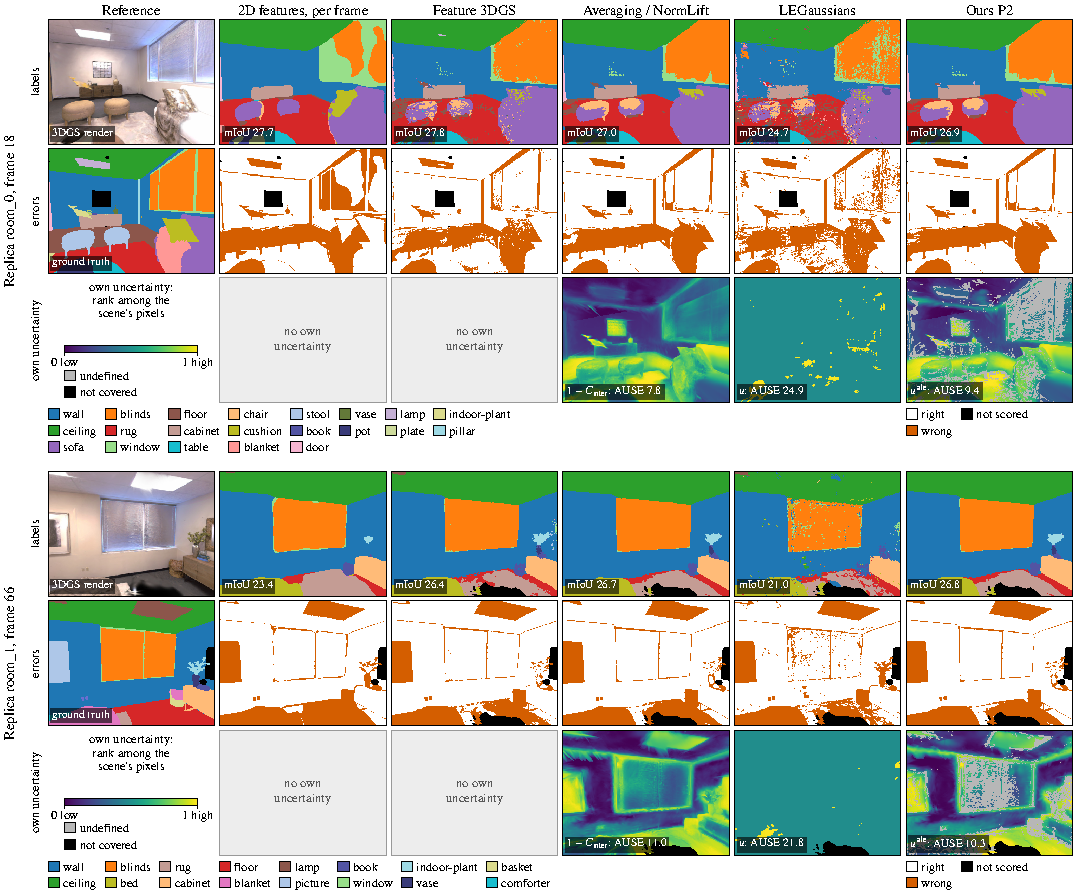
\includegraphics[width=\textwidth,page=1]{figs/supp_compare_all.pdf}
  \caption{Segmentation and own uncertainty of every method on Replica room\_0 (frame 18), Replica room\_1 (frame 66), Replica office\_1 (frame 25), Replica office\_2 (frame 75), Replica office\_3 (frame 15), Replica office\_4 (frame 29), ScanNet scene0070\_00 (frame 46), ScanNet scene0097\_00 (frame 2), ScanNet scene0140\_00 (frame 57), ScanNet scene0200\_00 (frame 36), ScanNet scene0347\_00 (frame 0), ScanNet scene0400\_00 (frame 0), ScanNet scene0590\_00 (frame 104) and ScanNet scene0645\_00 (frame 156). Every test scene, at the evaluation frame with the most ground-truth classes that cover at least 0.5\% of its labeled pixels (a rule on the labels only, fixed before rendering). Row 1: the 3DGS render and the labels (black: no decision); row 2: the ground truth and the errors (vermillion: wrong; black: not scored); row 3: each method's own uncertainty, NormLift's $1-C_{\mathrm{inter}}$, the learned $u$ of LEGaussians and our $u^{\mathrm{ale}}$, as its rank among the covered labeled pixels with a defined value in all evaluation frames of the scene (grey: undefined; black: not covered). The 2D features and Feature 3DGS have no own uncertainty (-- in Table~\ref{M-tab:replica}); we show no P2 confidence. Numbers are per-scene values over all evaluation frames, read from Table~\ref{M-tab:replica}: mIoU (row 1) and the AUSE of the own uncertainty (row 3), in \%. LEGaussians $\lambda_u$ = 4 (Replica), 1 (ScanNet), chosen on validation.}
  \label{fig:supp-grid}
\end{figure*}

\begin{figure*}[p]
  \centering
  \includegraphics[width=\textwidth,page=2]{figs/supp_compare_all.pdf}
  \caption{Continued from Fig.~\ref{fig:supp-grid}.}
\end{figure*}

\begin{figure*}[p]
  \centering
  \includegraphics[width=\textwidth,page=3]{figs/supp_compare_all.pdf}
  \caption{Continued from Fig.~\ref{fig:supp-grid}.}
\end{figure*}

\begin{figure*}[p]
  \centering
  \includegraphics[width=\textwidth,page=4]{figs/supp_compare_all.pdf}
  \caption{Continued from Fig.~\ref{fig:supp-grid}.}
\end{figure*}

\begin{figure*}[p]
  \centering
  \includegraphics[width=\textwidth,page=5]{figs/supp_compare_all.pdf}
  \caption{Continued from Fig.~\ref{fig:supp-grid}.}
\end{figure*}

\begin{figure*}[p]
  \centering
  \includegraphics[width=\textwidth,page=6]{figs/supp_compare_all.pdf}
  \caption{Continued from Fig.~\ref{fig:supp-grid}.}
\end{figure*}

\begin{figure*}[p]
  \centering
  \includegraphics[width=\textwidth,page=7]{figs/supp_compare_all.pdf}
  \caption{Continued from Fig.~\ref{fig:supp-grid}.}
\end{figure*}

\section{Agreement estimator}
\label{supp:plane}
Fig.~\ref{fig:plane} illustrates the estimator~\eqref{M-eq:rho} of \secref{M-sec:uncertainty} on simulated views: it keeps little evidence and conflicting evidence apart, which the mean resultant length and the prior-shrunk agreement do not.

\begin{figure}[t]
  \centering
  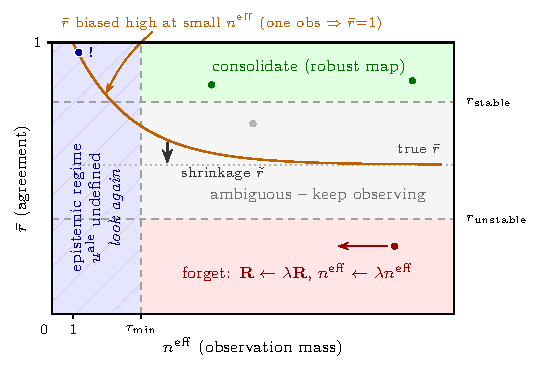
\includegraphics[width=\linewidth]{figs/uncertainty_plane.pdf}
  \caption{Support $s$ (weighted views) against agreement $\hat\rho$ of one Gaussian. The curves are root-mean-square values for two Gaussians with true agreement $\rho$ (dotted). The mean length $\lVert\R\rVert/W_1$ makes the conflicting one look consistent at few views, and the shrunk $\lVert\R\rVert/(W_1+c_0)$ makes the consistent one look conflicting. Our $\hat\rho$ ($\hat\rho^2$ is unbiased before the clamp) stays close to $\rho$. A fired change test resets $s$ to at most one view.}
  \label{fig:plane}
\end{figure}

\section{Fitted temperatures and build cost}
\label{supp:cost}
Table~\ref{tab:p2} lists the fitted P2 coefficients; on ScanNet $\gamma_e$ and $\gamma_a$ are negative. Table~\ref{tab:cost} gives the build time per ScanNet scene from the production logs of a shared RTX~4070~Ti, so the times include contention with other jobs.

\begin{table}[t]
\centering
\caption{P2 coefficients fitted by NLL on the validation scenes, and the temperature $\beta$ of P0.}
\label{tab:p2}
\footnotesize
\begin{tabular}{@{}lccccc@{}}
\toprule
Dataset & $\beta_0$ & $\gamma_e$ & $\gamma_a$ & $\gamma_u$ & $\beta$ (P0)\\
\midrule
%% generated by scripts/quant_stats.py (commands in docs/reports/2026-10-20-figures-video/logs/quant_summary.md)
Replica & 45.6 & +0.36 & +11.83 & +0.055 & 36.0\\
ScanNet & 34.6 & -0.80 & -2.06 & +0.142 & 39.2\\
\bottomrule
\end{tabular}
\end{table}

\begin{table*}[t]
\centering
\caption{Build time per ScanNet scene in seconds, median (min--max) over the ten scenes. Top: per step. Bottom: end to end with the shared 3D-GS fit and LSeg, and the per-scene ratio to ours.}
\label{tab:cost}
\footnotesize
\setlength{\tabcolsep}{3pt}
\begin{tabular}{@{}llc@{}}
\toprule
Method & Step & Seconds\\
\midrule
%% generated by scripts/quant_stats.py (commands in docs/reports/2026-10-20-figures-video/logs/quant_summary.md)
Ours, averaging, NormLift & field update, one pass (view hooks) & 5.6 (3.0--27.4)\\
Every method & LSeg extraction & 13.5 (5.7--48.4)\\
Every method & 3DGS map fit & 324.3 (266.6--694.5)\\
Feature 3DGS (re-impl.) & feature training, fixed map & 1267.5 (740.0--2037.0)\\
LEGaussians (re-impl.) & feature training, fixed map & 730.0 (385.0--1375.0)\\
\midrule
Method & Seconds & Ratio\\
\midrule
Ours, averaging, NormLift & 346 (282--716) & reference\\
Feature 3DGS (re-impl.) & 1614 (1051--2748) & 4.0 (3.0--6.6)\\
LEGaussians (re-impl.) & 1078 (782--2086) & 2.9 (1.8--5.3)\\
\bottomrule
\end{tabular}
\end{table*}



\textbf{Run time per keyframe.} On one Replica validation scene (NVIDIA RTX 4070 Ti, Intel Core i7-13700KF, no other job), a keyframe takes $109.9\pm7.6$\,ms: $69.9\pm2.7$\,ms for LSeg, $20.4\pm6.0$\,ms for the render and backward pass, and $16.7\pm2.4$\,ms for the statistics, change test and re-admission. Peak GPU memory is 1.9\,GiB; averaging and NormLift reuse our sums and add $2.3$\,ms; the field state takes 844 bytes per Gaussian. Fitting a Replica map took $4.5\pm0.6$\,min on an RTX 5070 Ti.
\section{Registered later attempts}
\label{supp:attempts}
After the first version of the results, we tried five changes meant to improve them. Each was registered before it ran, chosen on the validation scenes by a rule fixed in advance and, where validation selected it, run once on the test scenes. None improved on the paper's method, which therefore stays unchanged; Table~\ref{tab:attempts} gives the outcomes.

\begin{table*}[t]
\centering
\caption{Registered later attempts. Validation scenes select; the test scenes run once after the selection. Stale answers: share of the removed object's covered pixels still answering its query (\%).}
\label{tab:attempts}
\footnotesize
\setlength{\tabcolsep}{3pt}
\begin{tabular}{@{}p{0.2\textwidth}p{0.37\textwidth}p{0.37\textwidth}@{}}
\toprule
Attempt & Validation & Test\\
\midrule
%% sources: docs/reports/2026-10-17-paper-completion (attempts 03, 03b), docs/reports/2026-10-20-figures-video
%% (attempts 01-04; logs/{smooth_stage1,reset_fused_stage1,fusion_stage1,extractor_stage1}.md)
Vote predictive from the same posterior (with a P1 prior grid and P2 on P1) & Replica pooled NLL: P2 0.800, best alternative 0.809; P2 kept on both datasets & not selected; disclosed second look on Replica: vote predictive ECE 6.3, NLL 1.06, AURC 16.4 (P2: 8.7, 1.00, 12.2)\\
Pooling each Gaussian's statistics over its 3D neighbors (24 Gaussian kernels) & Replica: no kernel beats P2; ScanNet: a kernel selected (NLL 0.403 vs 0.410) & ScanNet NLL 0.535 vs 0.509 (P2) and 0.512 (averaging); ECE 6.6 vs 6.1, 6.2; AURC 5.4 vs 5.0, 4.4\\
Fused detectors fire the reset (our test with the feature and depth residuals) & stale answers 24.1 vs 24.8 (ours); Gaussian AP of the firing score 85.7 vs 60.3 & stale answers 26.0 vs 20.7, lower in 3 of 10 scenes; firing AP 79.3 vs 53.4; FA 3.7 vs 6.2\\
Fusing the map with the current frame, weighted by $u^{\mathrm{epi}}$ and $u^{\mathrm{ale}}$ & Replica: every fused row +1.4 mIoU; ours best NLL & fused rows change mIoU by at most 0.4; ours worse than a constant weight in 11 of 14 scenes (mIoU, NLL)\\
Stronger extractor for every row (RADSeg, ProxyCLIP ViT-H, Trident) & 2D mIoU Replica / ScanNet: LSeg 30.8 / 67.5, RADSeg 34.0 / 43.1, ProxyCLIP 26.1 / 38.0, Trident 29.4 / 35.9 & not run: no candidate gained on both datasets\\
\bottomrule
\end{tabular}
\end{table*}

\clearpage   % flush the figures and tables before the references
\bibliographystyle{IEEEtran}
\bibliography{ref}

\end{document}
